\section{Introduction} \label{sec:intro}

\subsection{Background} \label{sec:background}
With a higher than ever number for devices connected to the internet than ever\cite{iot_stats}, more devices are vulnerable than ever. Many do not want a wireless lock on their house, since there is a chance it can be hacked by malicious parties. The lock must of course be secure and resistant to attacks, but it is hard to create something that is a hundred percent secure. The same challenge is even more important for industrial systems, where loss of money, damage to the environment or even loss of life can be the consequences of system failure. There are already many examples of cyber-attacks on industrial systems, for example STRUXNET\cite{struxnet}, a computer worm that infected an Iranian nuclear facility. 
As with other industries, the marine and offshore industries are connecting more parts of their Cyber-Physical Systems(CPS) to the internet to improve their efficiency. While a lot of the Cyber-Physical Systems connected to the internet are well maintained and secure, many others are vulnerable. This is most often because the CPSs are not set up properly or run outdated software. Other than this, it is a "fact" of statistics that if a quantity Cyber-Physical Systems are connected to the internet, a portion of these will be insecure. 

The IT security standard for industrial communication networks, IEC62443 describes preliminary recommendations and guidance for the use of cybersecurity technology and countermeasures. To stay as secure as possible, the industries should apply these measures.\cite{IEC62443} Among other things, it specifies that firewalls should be added to systems that have the ability to "[Filter] IP-addresses on the outside allowed on the inside and vice versa". And filter "[ports and] applications allowed for communication". In other words, only devices that have a good reason for being connected to the Internet should be connected. 

DNV-GL is an independent expert in risk management and quality assurance, and has a big portion of their focus is on the maritime and offshore business. The DNV-GL has a Cyber Security team that helps customers assess and manage risks related to cyber security,~\cite{DNVGL_cybersec} and might have a interest in the findings of this project.

The research in cybersecurity at NTNU is mostly done at the Department of Information Security and Communication Technology and  the Department of Computer Science. As cybersecurity is important, some focus should be put on the topic at other departments as well, where it is relevant. This is the case for the Department of Engineering Cybernetics, which have a lot of focus on computer systems, both for the industry and embedded systems. Project theses like this one can be a way for the departments to get more insight in the importance of cybersecurity.

\subsection{Objectives}
The goal of this project is to map of Cyber-Physical Systems(CPS) in the maritime and offshore industry that is reachable through the internet, and by doing so get an overview of the exposure of these cyber-physical systems.

This goal was split into tasks, which define that this project should
\begin{enumerate}
    \item Introduce and define some key terms and concepts related to cybersecurity
    \item Explain what is meant by a cyber-physical system and why cybersecurity is a topic of concern for such systems.
    \item Identify and explain search tools that can be used to identify publicly cyber-physical systems, with the focus on the equipment and systems used in the maritime and offshore oil and gas industry. 
    \item Prepare a specification for how a search can be carried out in one or more of the identified tools. Explain the rationales for the choices made in relation to the search, for example for delimiting the outcomes.
    \item Document the results from applying the tools and elaborate on the findings.
    \item Identify potential topics that may require further research, based on the findings and in collaboration with the supervisors.
\end{enumerate}


Open-source intelligence(OSINT) is utilized to map the CPS. The OSINT search engine \href{https://shodan.io}{\color{blue}{Shodan}}\cite{shodan} is a popular search engine for enumerating Internet-connected systems, and will be used as the main reconnaissance tool of this project. 
Since all publicly available devices is already mostly scanned and indexed by Shodan, the difficult part will be to recognize devices within the constraints of CPS in the maritime and offshore industries.


\subsection{Limitations and assumptions} \label{sec:limits}
In \cref{sec:ipv6} it is assumed that industries in the offshore and maritime industries will not use a significant amount of IPv6. This is based on the findings from when this report is written, and the situation will hopefully change in the coming years. However, due to this, IPv6 was not investigated as thoroughly as IPv4.

Shodan is used as the main OSINT tool in this report. Any shortcomings of this tool will also affect the work of this project.

There are other tools available as well. Some of them has the same functionality as Shodan, like \href{https://censys.io/}{\color{blue}{Censys}}\cite{censys} and \href{www.zoomeye.org}{\color{blue}{ZoomEye}}\cite{zoomeye}. Other tools, like the Traceroute tool used in \cref{sec:latency_method}, covers functionality that Shodan does not. There is many available OSINT tools available, and while Shodan was assessed to be the most fitting to this project, parts of it might be easier or more efficient to do with other tools. Tools not mentioned in the report were either not found or evaluated as not relevant.

Honeypot technology is to make a computer pretend to be another device. This is often done to do statistics on attempts to access the impersonated systems are done. This technology is quite popular for use on CPS, and during the research of this project, multiple other articles were found that set up honeypots as part of their research.\cite{bodenheim_butts_dunlap_mullins_2014}\cite{ICS_shodan_article} There is therefore a chance that some of the devices found by Shodan are in reality fake. Shodan has a function for identifying honeypots, but it is not foolproof.

A device connected to the internet might have multiple different IP addresses associated with it. In this project, it is assumed that every IP address is a single device, as this is usually the case.


\subsection{Research approach} \label{sec:research_approach}
The work of this project will mostly be intelligence: To suggest methods for detecting devices as per the project goal. In this report, all mentions of "method" will refer to these methods.
To achieve the project goal in an efficient way, an approach is followed.
The first step will be to get familiar with the Open-source Intelligence tools useful for the purpose of identifying and analyzing devices connected to the internet. 

Research will be made to see what methods already exist. These methods will be tested with the constraints. Then the supervisors from both DNV-GL and NTNU will be consulted for thoughts on the methods found. Changes will be made to the methods according to the feedback. Then both the iterations of the methods will be tested again. Based on the new results, individual research is again performed, thus completing the loop illustrated in \cref{fig:workflow} This process will be repeated until the interested parties are satisfied. 
The main focus of this research approach is to identify and suggest existing methods.

The research mentioned in this approach was mostly done by reading articles on the subject. These articles were found by using the search engines Engineering Village\cite{engineering_village} and Google Scholar\cite{google_scholar}. During the research, however, it was found that some OSINT techniques was easier to find in online blogs. These were found by utilizing the DuckDuckGo internet search engine\cite{ddg}. 


\tikzset{every picture/.style={line width=0.75pt}}
 
\begin{tabular}{p{10cm}}

    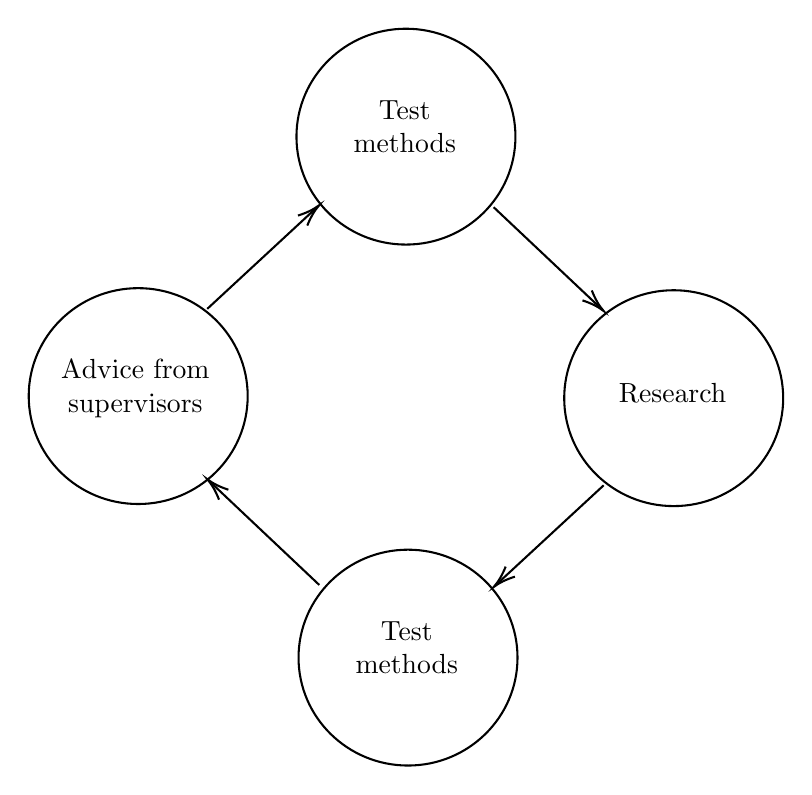
\begin{tikzpicture}[x=0.75pt,y=0.75pt,yscale=-1,xscale=1]
        %uncomment if require: \path (0,427); %set diagram left start at 0, and has height of 427

        %Shape: Ellipse [id:dp8381675984532289] 
        \draw   (107.5,211) .. controls (107.5,182.28) and (131.12,159) .. (160.25,159) .. controls (189.38,159) and (213,182.28) .. (213,211) .. controls (213,239.72) and (189.38,263) .. (160.25,263) .. controls (131.12,263) and (107.5,239.72) .. (107.5,211) -- cycle ;
        %Shape: Ellipse [id:dp8879090651544747] 
        \draw   (236.5,86) .. controls (236.5,57.28) and (260.12,34) .. (289.25,34) .. controls (318.38,34) and (342,57.28) .. (342,86) .. controls (342,114.72) and (318.38,138) .. (289.25,138) .. controls (260.12,138) and (236.5,114.72) .. (236.5,86) -- cycle ;
        %Shape: Ellipse [id:dp159469530573498] 
        \draw   (365.5,212) .. controls (365.5,183.28) and (389.12,160) .. (418.25,160) .. controls (447.38,160) and (471,183.28) .. (471,212) .. controls (471,240.72) and (447.38,264) .. (418.25,264) .. controls (389.12,264) and (365.5,240.72) .. (365.5,212) -- cycle ;
        %Shape: Ellipse [id:dp6243045365348194] 
        \draw   (237.5,337) .. controls (237.5,308.28) and (261.12,285) .. (290.25,285) .. controls (319.38,285) and (343,308.28) .. (343,337) .. controls (343,365.72) and (319.38,389) .. (290.25,389) .. controls (261.12,389) and (237.5,365.72) .. (237.5,337) -- cycle ;
        %Straight Lines [id:da3764417411513329] 
        \draw    (193.5,169) -- (246.03,120.36) ;
        \draw [shift={(247.5,119)}, rotate = 497.2] [color={rgb, 255:red, 0; green, 0; blue, 0 }  ][line width=0.75]    (10.93,-3.29) .. controls (6.95,-1.4) and (3.31,-0.3) .. (0,0) .. controls (3.31,0.3) and (6.95,1.4) .. (10.93,3.29)   ;
        %Straight Lines [id:da08718773032378624] 
        \draw    (384.5,254) -- (332.97,301.64) ;
        \draw [shift={(331.5,303)}, rotate = 317.25] [color={rgb, 255:red, 0; green, 0; blue, 0 }  ][line width=0.75]    (10.93,-3.29) .. controls (6.95,-1.4) and (3.31,-0.3) .. (0,0) .. controls (3.31,0.3) and (6.95,1.4) .. (10.93,3.29)   ;
        %Straight Lines [id:da9455012657988889] 
        \draw    (331.5,120) -- (383.05,168.63) ;
        \draw [shift={(384.5,170)}, rotate = 223.32999999999998] [color={rgb, 255:red, 0; green, 0; blue, 0 }  ][line width=0.75]    (10.93,-3.29) .. controls (6.95,-1.4) and (3.31,-0.3) .. (0,0) .. controls (3.31,0.3) and (6.95,1.4) .. (10.93,3.29)   ;
        %Straight Lines [id:da04085276077852196] 
        \draw    (247.5,302) -- (194.95,252.37) ;
        \draw [shift={(193.5,251)}, rotate = 403.36] [color={rgb, 255:red, 0; green, 0; blue, 0 }  ][line width=0.75]    (10.93,-3.29) .. controls (6.95,-1.4) and (3.31,-0.3) .. (0,0) .. controls (3.31,0.3) and (6.95,1.4) .. (10.93,3.29)   ;

        % Text Node
        \draw (259.25,67) node [anchor=north west][inner sep=0.75pt]   [align=left] {\begin{minipage}[lt]{41.865356pt}\setlength\topsep{0pt}
            \begin{center}
                Test \\methods
            \end{center}

        \end{minipage}};
        % Text Node
        \draw (117.75,192) node [anchor=north west][inner sep=0.75pt]   [align=left] {\begin{minipage}[lt]{59.42064400000001pt}\setlength\topsep{0pt}
            \begin{center}
                Advice from \\supervisors
            \end{center}

        \end{minipage}};
        % Text Node
        \draw (385.25,203.5) node [anchor=north west][inner sep=0.75pt]   [align=left] {\begin{minipage}[lt]{46.398644000000004pt}\setlength\topsep{0pt}
            \begin{center}
                Research
            \end{center}

        \end{minipage}};
        % Text Node
        \draw (260.25,318) node [anchor=north west][inner sep=0.75pt]   [align=left] {\begin{minipage}[lt]{41.865356pt}\setlength\topsep{0pt}
            \begin{center}
                Test \\methods
            \end{center}

        \end{minipage}};


    \end{tikzpicture}

    \captionof{figure}{Illustration of workflow}
    \label{fig:workflow}
\end{tabular}



\subsection{Structure of report}
This report has five main parts. First, in this section, \cref{sec:intro}, the project is introduced. In \cref{sec:theory}, basic principles used in this project is explained. Important principles from the working of the internet is explained, along with the basics of the Shodan search engine. In \cref{sec:method} different methods for selective identification of IP devices are outlined. In \cref{sec:results} the results from using the aforementioned methods are listed, along with discussion of these results. In \cref{sec:conclusion} a conclusion is drawn from the results.  Lastly, suggestions for further work on the topic is suggested

\newpage
